\documentclass[9pt,twocolumn,twoside]{styles/osajnl}
\usepackage{fancyvrb}
\journal{i524} 

\title{Ceph - Distributed Storage System}

\author[1]{Rahul Raghatate}
\author[1]{Snehal Chemburkar}

\affil[1]{School of Informatics and Computing, Bloomington, IN 47408, U.S.A.}

\affil[*]{Corresponding authors: rragahta@iu.edu, snehchem@iu.edu }

\dates{paper-1, \today}

\ociscodes{Ceph, scalability, storage, exabytes}

% replace this with your url in github/gitlab
\doi{\url{https://github.com/rahulraghatate/sp17-i524/paper1/S17-IR-2026/report.pdf}}


\begin{abstract}
Ceph  is a unique storage solution that delivers all critical storage system capabilities:open-source, software-defined, enterprise-class and unified storage (object, block, file). Ceph being highly reliable, easy to manage and free, possesses  power to transform company’s IT infrastructure and ability to manage vast amounts of data. Ceph's extraordinary scalability has provided clients with accessibility to  petabytes to exabytes of data. Moreover basic enterprise storage features including: replication (or erasure coding), snapshots, thin provisioning, auto-tiering (ability to shift data between flash and hard drives), self-healing capabilities has resulted in allowing it to be a reliable big data storage platform. This article explores these salient features Ceph as well as provides study of Ceph architecture and its uniqueness in comparison to few of the existing Large Scale Systems.  
\newline
\end{abstract}

\setboolean{displaycopyright}{true}

\begin{document}

\maketitle

\section{Introduction}

Developing a distributed file system(DFS) in today's world of
exponentially growing data is not a handy job. However, if the right issues
are addressed and resolved, it becomes immensely valuable and
foundation stone in any business success. Although most of the DFS
offer a similar set of features, they also can provide unique features
which allow them to stand distinct.

For IT Decision Makers, inadequate storage infrastructure stand out to
be the fourth out of the top ten pain points. It's interesting to know
that 74\% of IT decision makers are worried about their organization’s
ability to cope with an increasing volume of data, and 70\% believe
that their current storage systems will not be able to handle next
generation workloads \cite{ceph-redhat-datasheet}. Hence, Enterprises
in due struggle to manage the explosive growth of data while remaining
agile and cost competitive are turning to cloud technology to store
their data.

As a self-healing, self-managing platform with no single point of
failure, Red Hat Ceph Storage significantly lowers the cost of storing
enterprise data in the cloud and helps enterprises manage their
exponential data growth in an automated fashion
\cite{ceph-redhat-datasheet}.

Ceph is open-source storage platform providing highly scalable object,
block as well as file-based storage. It is a unified, distributed storage system designed for excellent performance, reliability and scalability \cite{www-ceph}.

Ceph has emerged as one of the best storage ecosystem which initially began as a PhD research project in storage systems by Sage Weil at the University of California, Santa Cruz (UCSC). The name Ceph comes from Cephalopod, a class of mollusks.


\section{Architecture}

The Ceph architecture consists of four subsystems:
\begin{itemize}
\item File System Clients
\item Cluster of metadata servers(MDS)
\item RADOS which includes Monitor Services and object storage
  devices(OSDs)
\item Data distribution system using CRUSH
\end{itemize}

\begin{figure}[htbp]
\centering
\fbox{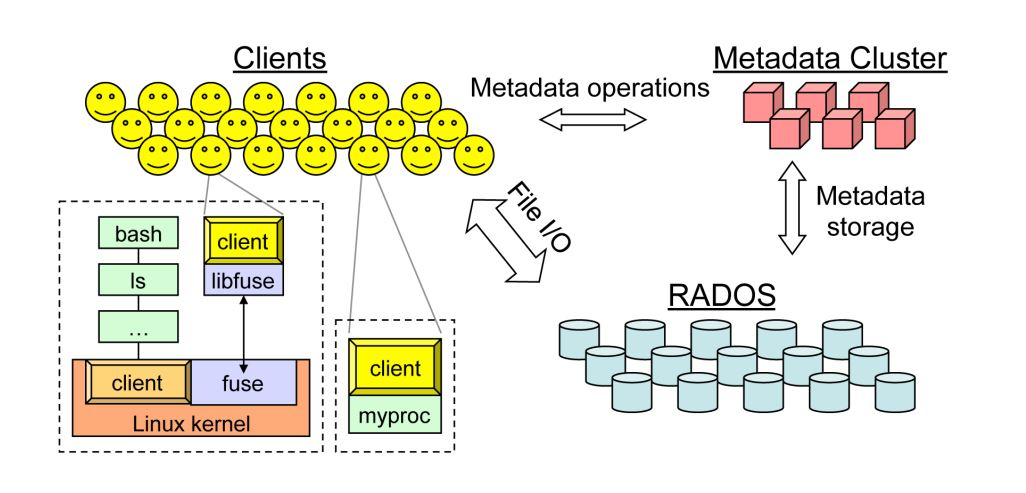
\includegraphics[width=\linewidth]{images/Ceph-System-Layout}}
\caption{System Layout of Ceph \cite{paper-Ceph}}.
\label{CSL}
\end{figure}

\subsection{Client Operation} 
Ceph depends upon Ceph Clients and Ceph OSD Daemons having knowledge
of the cluster topology, which is inclusive of 5 maps collectively
referred to as the “Cluster Map”.The Ceph Client is the user of the
Ceph file system. The Ceph client runs on each host executing
application code and exposes a file system interface to
applications. Ceph has a user-level client as well as a kernel
client. The user-level client is either linked directly to the
application or used via FUSE. The kernel client allows the Ceph file
system to be mounted. Each client maintains its own file data cache,
independent of the kernel page or buffer caches, making it accessible
to applications that link to the client directly \cite{paper-Ceph}.
\subsection{The Ceph metadata server(MDS)}
Ceph provides a cluster of metadata servers which continually
load-balances itself using dynamic subtree partitioning
\cite{ceph-metadata}. The responsibility for managing the namespace
hierarchy is adaptively and intelligently distributed among tens or
even hundreds of metadata servers. The key to the MDS cluster’s
adaptability is that Ceph metadata items are very small and can be
moved around quickly. To enable failure recovery, the MDS journals
metadata updates to OSDs. The mapping of metadata servers to namespace
is performed in Ceph using dynamic subtree partitioning, which allows
Ceph to adapt to changing workloads (migrating namespaces between
metadata servers) while preserving locality for
performance. Rebalancing of the MDS at even extreme workload changes
is usually accomplished within a few seconds. Clients are notified of
relevant partition updates whenever they communicate with the MDS
\cite{www-ibm-ceph}.

\begin{figure}[htbp]
\centering
\fbox{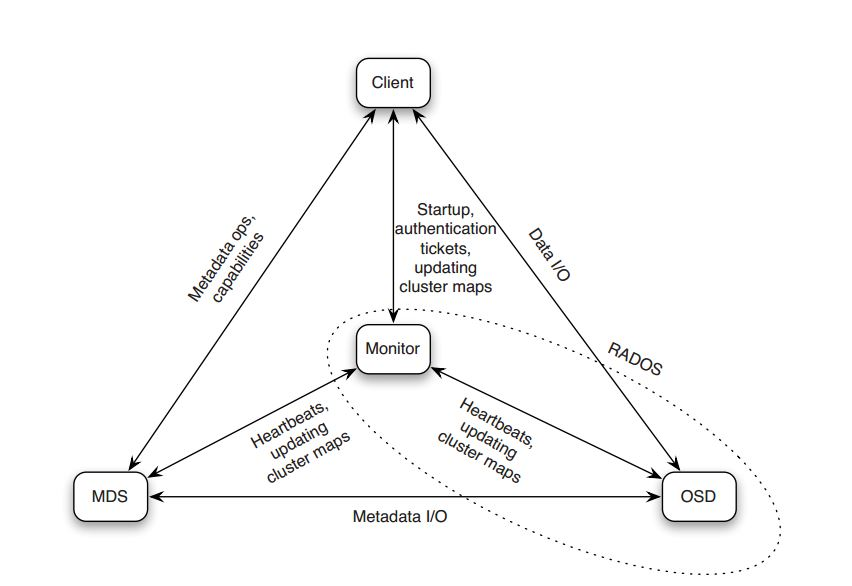
\includegraphics[width=\linewidth]{images/Ceph-Components-Interaction}}
\caption{Ceph components interaction \cite{paper-ceph-hadoop}.}
\label{CCI}
\end{figure}

\subsection{Reliable Autonomic Distributed Object Storage (RADOS)}
From a bird view, object storage cluster made of hundreds of thousands
of OSDs as a single logical object store and namespace to the Ceph
clients and metadata servers. Ceph’s RADOS achieves linearity in both
capacity and aggregated performance by delegating management of object
replication, cluster expansion, failure detection and recovery to OSDs
in a distributed fashion. RADOS can also be used as a stand-alone
system.

Unlike other parallel file systems, replication is managed by OSDs
instead of clients, which shifts replication bandwidth overhead to the
OSD cluster, simplifies the client protocol, and provides fully
consistent semantics in mixed read/write workloads. RADOS manages the
replication of data using a variant of primary-copy replication and
replicas are stored in placement groups which includes a primary OSD
which serializes all requests to the placement group.

Writes are applied in two phases and this approach separates writing
for the purpose of sharing with other clients from writing for the
purpose of durability and makes sharing data very fast. Ceph’s failure
detection and recovery are fully distributed. The monitor service is
only used to update the master copy of the cluster map. OSDs
communicates the cluster map updates using epidemic-style propagation
that has bounded overhead. This procedure is used to respond to all
cluster map updates, whether due to OSD failure, cluster contraction,
or expansion. OSDs always collaborate to realize the data distribution
specified in the latest cluster map while preserving consistency of
read/write access \cite{paper-ceph-hadoop}.

\subsection{Data Distribution System}
The small size of metadata items in the MDS and the compactness of
cluster maps in RADOS are enabled by CRUSH (Controlled Replication
Under Scalable Hashing) \cite{MDS}. Ceph uses this hash function to
calculate the placement of data instead of using allocation tables,
which can grow very large and unwieldy. CRUSH is part of the cluster
map and behaves like a consistent hashing function in that failure,
removal, and addition of nodes result in near-minimal object migration
to re-establish near-uniform distribution. CRUSH maps a placement
group ID to an ordered list of OSDs, using a hierarchically structured
cluster map and placement rules as additional input. Any list output
by CRUSH meets the constraints specified by placement rules preventing
two replicas being placed in same failure domain
\cite{paper-Ceph}. Knowledge of failure domains is important for
overall data safety of very large storage systems where correlated
failures are common.

\section{Salient Features}
\begin{enumerate}
\item Ceph Clients include several service interfaces. These include:
\begin{itemize}
\item Block Devices: The Ceph Block Device (a.k.a., RBD) service
  provides resizable, thin-provisioned block devices with snapshotting
  and cloning.
\item Object Storage: The Ceph Object Storage (a.k.a., RGW) service
  provides RESTful APIs with interfaces that are compatible with
  Amazon S3 and OpenStack Swift.
\item Filesystem: The Ceph Filesystem (CephFS) service provides a
  POSIX compliant filesystem usable with mount or as a filesytem in
  user space (FUSE).
\end{itemize}
\item Scalability and high availability: In traditional architectures
  there is single point of entry to a complex subsystem. This imposes
  a limit to both performance and scalability, while introducing a
  single point of failure.  Ceph eliminates the centralized gateway
  using CRUSH algorithm to enable clients to interact with Ceph OSD
  Daemons directly. Ceph OSD Daemons create object replicas on other
  Ceph Nodes to ensure data safety and Ceph Monitors provide high
  availability \cite{www-ceph-scalable}.
\item Network Security: Ceph provides its cephx authentication system
  to authenticate users and daemons. Cephx uses shared secret keys for
  mutual authentication, such that both parties can prove to each
  other they have a copy of the key without actually revealing it.
\item Dyanamic cluster management: Ceph uses CRUSH which enables
  modern cloud storage infrastructures to place data, re-balance the
  cluster and recover from faults dynamically. The Ceph storage system
  supports the notion of ‘Pools’, which are logical partitions for
  storing objects.
\item Smart Daemons enable hyperscale \cite{www-ceph-daemon}: The
  ability of Ceph Clients, Ceph Monitors and Ceph OSD Daemons to
  interact with each other allows Ceph OSD Daemons to utilize the CPU
  and RAM of the Ceph nodes perform task easily that can bog down a
  centralized server.Leveraging this computing power leads to several
  major benefits:
\begin{itemize}
\item OSDs Service Clients Directly: Ceph Clients can maintain a
  session when they need to, and with a certain Ceph OSD Daemon
  instead of a centralized server.
\item OSD Membership and Status: The Ceph OSD Daemon status reflects
  whether it is running and able to service Ceph Client requests. Ceph
  also empowers OSD Daemons with ability to check each other's
  heartbeats and report back to the Ceph Monitor reliving their
  burden.
\item Data Scrubbing: Ceph OSD Daemons insures data integrity by
  scrubbing placement groups.Light scrubbing (daily) catches bugs or
  filesystem errors. Deep scrubbing (weekly) finds bad sectors on a
  drive that weren’t apparent in a light scrub.
\item Replication:Like Ceph Clients, Ceph OSD Daemons use the CRUSH
  algorithm, but the Ceph OSD Daemon uses it to compute where replicas
  of objects should be stored (and for rebalancing).
\begin{figure}[htbp]
\centering
\fbox{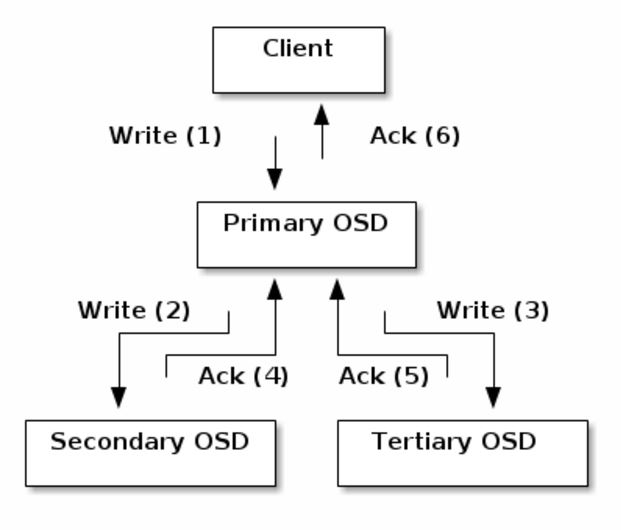
\includegraphics[width=\linewidth]{images/Replication-Process}}
\caption{Replication Process \cite{www-ceph-daemon}.}
\label{RP}
\end{figure}

\end{itemize}
\item Ceph’s provides a native interface to the Ceph Storage Cluster
  via librados, and a number of service interfaces built on top of
  librados.
\end{enumerate}

\section{Related Work}
Ceph scalability provide high-performance access to a small set of
files by tens of thousands of cooperating clients in contrast to
Largescale systems like OceanStore \cite{paper-oceanstore} and Farsite
\cite{paper-farsite} which fails due to bottlenecks in subsystems such
as name lookup. Ceph proves more reliable over other parallel file and
storage systems such as Vesta \cite{paper-vesta}, Galley
\cite{paper-gallery}, PVFS \cite{mag-pvfs}, and Swift
\cite{report-Swift} due to their lack of strong support for scalable
metadata access or robust data distribution. These systems also
typically suffer from block allocation issues: blocks are either
allocated centrally or via a lock-based mechanism, preventing them
from scaling well for thousands of write requests.

\section{Use Cases}
Ceph is being used in wide range of applications
\cite{www-ceph-usecases}. Few of them are listed below:
\begin{enumerate}
\item Red Hat Ceph Storage team worked with WDLabs and SuperMicro and
  built and tested a 504 node Ceph cluster with 4 PB of raw storage
  using these WDlabs Micro-Servers. \cite{wdlabs-ceph}.
\item Cloud Infrastructure for Microbial Bioinformatics (CLIMB) has
  selected and implemented Red Hat Ceph Storage for their large-scale
  extensive research needs \cite{climb-ceph}.
\item Yahoo's deployment of the community version of Ceph software for
  its Flickr and Mail applications on its Cloud Object Store (COS)
  \cite{yahoo-ceph-deploy}.
\item Red Hat Ceph Storage on Dell PowerEdge server
\item Red Hat Ceph Storage on Intel processors and SSDS
\end{enumerate}

\section{Useful Resources}
Ceph installation manual \cite{www-ceph-install}, provides
Installation and Deployment guide which is excellent resource as
starter kit. Tutorial on Ceph Deployment by Alan
Johnson\cite{ceph-deploy-guide} , is a good tutorial about Ceph
deployment.

\section{Conclusion}
Ceph provides unique solution for the three critical challenges of
large scale storage systems—scalability, performance, and
reliability. CRUSH and RADOS provides Ceph with improved data safety,
ability to manage data replication, failure detection and recovery,
low-level disk allocation, scheduling, and data migration without
encumbering any central server(s). Ceph’s metadata management
architecture addresses one of the most vexing problems in highly
scalable storage of providing a single uniform directory hierarchy
obeying POSIX semantics \cite{paper-Ceph}. Thus, Ceph has proven to be
one stop solution for the large-scale storage system in today's Big
Data World.

\section*{Acknowledgements}

This work was done as part of the course "I524: Big Data and Open
Source Software Projects" at Indiana University during Spring
2017. Many thanks to Professor Gregor von Laszewski and Prof. Geoffrey
Fox at Indiana University Bloomington for their academic as well as
professional guidance. We would also like to thank Associate
Instructors for their help and support during the course.

\bibliography{references}

\end{document}
